% \documentclass[a4paper, twocolumn]{article}
% \usepackage[fontsize=12.3pt]{fontsize}
% \usepackage{geometry}
% \usepackage[T1, T2A]{fontenc}
% \usepackage[utf8]{inputenc}
% \usepackage[russian]{babel}
% \usepackage{multirow}
% \usepackage{amsmath}
% \usepackage{titleps}
% \usepackage{graphicx}
% \usepackage[letterspace=200]{microtype}
% \usepackage{epstopdf}
% \usepackage{float}

% \geometry{
%     a4paper,
%     total={170mm,257mm},
%     left=20mm,
%     top=20mm,
% }

\setlength{\abovecaptionskip}{0pt plus 0pt minus 0pt}

\pagestyle{pagenumberfooterright}
\setcounter{page}{45}

% \begin{document}
% \begin{minipage}[t]{0.485\textwidth}

% \graphicspath{.}

\newcommand{\Cm}{\mbox{\usefont{T2A}{\rmdefault}{m}{n}\cyrs\cyrm}}
\newcommand{\M}{\mbox{\usefont{T2A}{\rmdefault}{m}{n}\cyrm}}

\noindent
в него входила только одна тригонометрическая функция угла $\alpha$. Для этого представим коэффициент трения k как тангенс некоторого угла $\varphi$:

\setlength{\abovedisplayskip}{-8pt} \setlength{\abovedisplayshortskip}{-8pt}

\begin{gather*}
\tg \varphi = k; \quad \varphi = \arctg k \\
\sin \varphi = \frac{k}{\sqrt{1+k^2}}; \quad \cos \varphi = \frac{k}{\sqrt{1+k^2}}.
\end{gather*}

Так как $k$ задано, угол $\varphi$ можно считать известным. Подставляя в (4) $\tg \varphi$ вместо $k$ и умножая числитель и знаменатель на $\cos \varphi$, получим

\begin{align*}
& F = \frac{P \tg \varphi}{\tg \varphi \sin \alpha + \cos \alpha} = \\
& = \frac{P \sin \varphi}{\sin \varphi \sin \alpha + \cos \varphi \cos \alpha}
= \frac{P \sin \varphi}{\cos(\alpha - \varphi)} = \\
& = \frac{Pk}{\sqrt{1+k^2} \cos(\alpha - \varphi)}.
\end{align*}

Теперь ясно, что сила $F$ будет минимальной тогда, когда $cos(\alpha - \varphi) = 1$, то есть

\[ a_{\min} = \varphi = \arctg k \]

При этом минимальное значение силы $F$ равно

\[ F_{\min} = \frac{kP}{\sqrt{1+k^2}} \]

Из решения этой задачи можно сделать практический вывод: когда необходимо везти на санях груз по дороге с большим коэффициентом трения (например, если дорога посыпана песком), нужно тянуть сани за короткую верёвку. Если же коэффициент трения мал, верёвка должна быть длинной. Объясните это.

\noindent
\textls{Задача 3.} \textit{Точки 1 и 2 движутся по осям x и y к началу координат (рис. 2). В момент $t_0 = 0$ точка 1 находится на расстоянии $s_1 = 10$ см,}

% \vspace{-10mm}

\noindent
\begin{figure}[H]
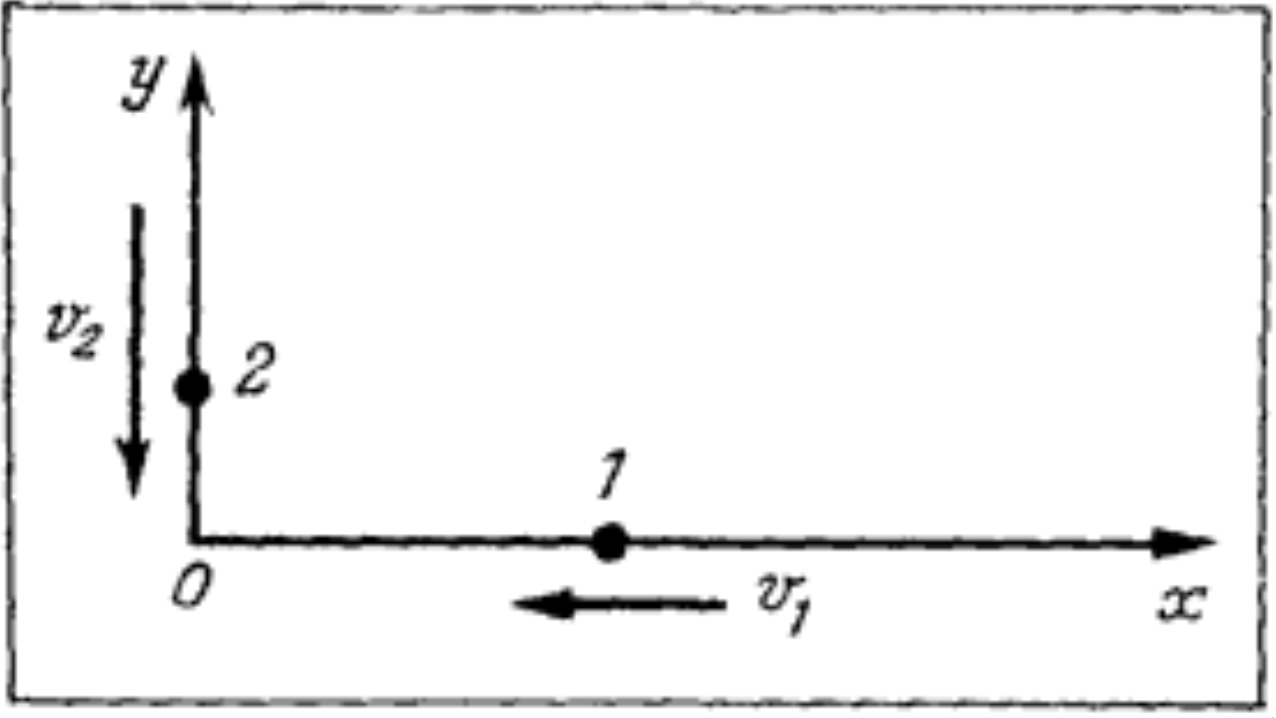
\includegraphics[scale=0.185]{img1.png}
\caption{}
\end{figure}

\noindent \textit{а точка 2 --- на расстоянии $s_2 = 5$ см от начала координат. Первая точка движется со скоростью $v_1 = 2$ см/с, а вторая --- со скоростью $v_2 = 4$ см/с. Каково наименьшее расстояние между ними?}

В момент времени $t$ расстояние между точками равно 

\begin{gather*}
d = \sqrt{(s_1 - v_1t)^2 + (s_2 - v_2t)^2} =\\
= \sqrt{(10 - 2t)^2 + (5 - 4t)^2} =\\
= \sqrt{20t^2 - 80t + 125} \, (\Cm).
\end{gather*}

Под корнем стоит квадратный трёхчлен, из которого можно легко выделить полный квадрат. Действительно,

\[ 20t^2 - 80t + 125 = 5 |(2t - 4)^2 + 9|. \]

Ясно, что минимум этого выражения, а значит и расстояния $d$ будет при $t = 2$, откуда

\[ d_{\min} = \sqrt{45} \, \Cm \approx 6,7 \, \Cm. \]

В заключение рассмотрим задачу, для решения которой используется так называемый метод приращений, не входящий в программу средней школы.

\textls{Задача 4.} \textit{Группа спорстменов организовала на берегу моря следующее соревновние. Стартуя из точки $A$ (рис. 3) на берегу моря, каждый спорстмен должен достичь буйка B, расположенного на расстоянии $l = 120 \, \M$ от берега. Береговую линию можно считать прямой; расстояние от старта A до основания перпендикуляра $BC$, опущенного на эту линию, равно $L = 200 \, \M$. Каждый спорстмен имеет право пробежать любое расстояние по берегу от старта $A$.}

\vspace{1mm}

\noindent
\begin{figure}[H]
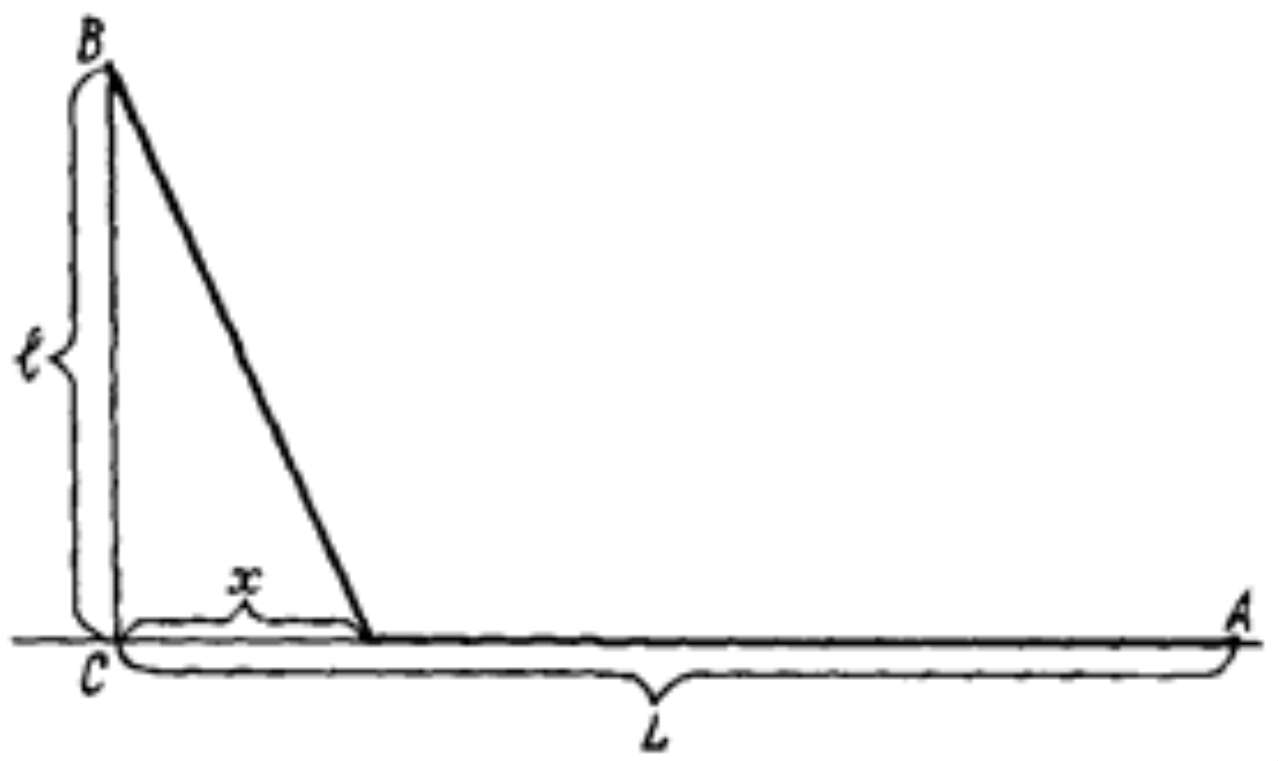
\includegraphics[scale=0.185]{img2.png}
\caption{}
\end{figure}

% \end{document}
